Οι δύο προηγούμενες ενότητες περιγράφουν μεθόδους ελάττωσης (α) του σφάλματος
εκτίμησης προσανατολισμού όταν η εκτίμηση θέσης συμπίπτει με τη θέση του
αισθητήρα, και (β) του σφάλματος εκτίμησης θέσης όταν η εκτίμηση
προσανατολισμού ισούται με τον προσανατολισμό του αισθητήρα. Ωστόσο στη γενική
περίπτωση καμία ισότητα δεν ισχύει. Επιπλέον το πρόβλημα είναι πεπλεγμένο: το
βέλτιστο σφάλμα προσανατολισμού δεν μπορεί να επιτευχθεί όταν το σφάλμα θέσης
δεν είναι μηδέν, και το βέλτιστο σφάλμα θέσης δεν μπορεί να επιτευχθεί όταν το
σφάλμα προσανατολισμού δεν είναι μηδέν (Παρατήρηση \ref{rem:iterative}).

Σε αυτή την ενότητα παρουσιάζουμε το γενικό σύστημα που είναι ικανό να
ενσωματώσει τις τρεις μεθόδους ελάττωσης του σφάλματος εκτίμησης
προσανατολισμού και τη μέθοδο ελάττωσης του σφάλματος εκτίμησης θέσης.  Το
προτεινόμενο σύστημα μειώνει στην αρχή το πρώτο είδος σφάλματος, και στη
συνέχεια το δεύτερο. Ως συνέπεια της παρατήρησης \ref{rem:iterative}, η
διαδικασία επαναλαμβάνεται μέχρι την ικανοποίηση συνθήκης τερματισμού. Η
μέθοδος αυτή περιγράφεται στα ακόλουθα.


%%%%%%%%%%%%%%%%%%%%%%%%%%%%%%%%%%%%%%%%%%%%%%%%%%%%%%%%%%%%%%%%%%%%%%%%%%%%%%%%
\subsection{Περιορισμοί των μεθόδων γωνιακής ευθυγράμμισης υπό γενικές συνθήκες}
\label{subsection:02_04_04:01}

Οι μέθοδοι εκτίμησης του προσανατολισμού της στάσης $\hat{\bm{p}}$ που
παρουσιάστηκαν στην ενότητα \ref{section:02_04_02} εμφανίζουν σε πραγματικές
συνθήκες περιορισμούς ως προς την τελική τους εκτίμηση.

Η μέθοδος Πρώτων Αρχών (ενότητα \ref{subsection:02_04_02:02}) εμφανίζει μη
προβλέψιμη και ασταθή συμπεριφορά όταν ο χάρτης του περιβάλλοντος δεν το
αναπαριστά τέλεια. Στο σχήμα \ref{fig:02_04_04:errorbar_x1} απεικονίζεται το
μέσο σφάλμα προσανατολισμού της μεθόδου Πρώτων Αρχών και η τυπική του απόκλιση
σε εκατό πειράματα. Στο αριστερό σχήμα ο χάρτης αναπαριστά στην εντέλεια το
περιβάλλον, σε αντίθεση με το δεξιό σχήμα, στο οποίο ο χάρτης είναι
διεφθαρμένος.

Εδώ παρατηρούμε ότι ενώ στην πρώτη περίπτωση το σφάλμα προσανατολισμού
αυξάνεται με συνέπεια για αυξανόμενο επίπεδο διαταραχών και μειώνεται με
συνέπεια για αυξανόμενο αριθμό εκπεμπόμενων ακτίνων, στη δεύτερη δεν εμφανίζει
καμία συνέπεια. Ταυτόχρονα παρατηρούμε τον μεγαλύτερο περιορισμό της μεθόδου,
ήτοι την αδιαφορία του σφάλματος ως προς τον αριθμό εκπεμπόμενων ακτίνων όταν
ο χάρτης δεν αναπαριστά τέλεια το περιβάλλον, η οποία είναι η γενική περίπτωση.
Αυτή η ιδιότητα είναι κρίσιμη γιατί η μέθοδος λειτουργεί στον συνεχή γωνιακό
χώρο και, σε αντίθεση με τις Προκρούστειες μεθόδους των ενοτήτων
\ref{subsection:02_04_02:01} και \ref{subsection:02_04_02:03}, δεν είναι δυνατή
η εφαρμογή \textit{εσωτερικής} μεθόδου επιπρόσθετης μείωσης των σφαλμάτων της,
όπως η μέθοδος του Θησέα. Συνεπώς είναι αναγκαία η εφεύρεση νέας μεθόδου,
εξωτερικής ως προς τη λογική της μεθόδου Πρώτων Αρχών για τη μείωση των
σφαλμάτων εκτίμησής της.


\begin{figure}[h]\centering
  \vspace{2cm}
  \definecolor{aa}{RGB}{200,200,200}
\definecolor{ab}{RGB}{161,218,180}
\definecolor{ac}{RGB}{65,182,196}
\definecolor{ad}{RGB}{44,127,184}

% GNUPLOT: LaTeX picture with Postscript
\begingroup
  \makeatletter
  \providecommand\color[2][]{%
    \GenericError{(gnuplot) \space\space\space\@spaces}{%
      Package color not loaded in conjunction with
      terminal option `colourtext'%
    }{See the gnuplot documentation for explanation.%
    }{Either use 'blacktext' in gnuplot or load the package
      color.sty in LaTeX.}%
    \renewcommand\color[2][]{}%
  }%
  \providecommand\includegraphics[2][]{%
    \GenericError{(gnuplot) \space\space\space\@spaces}{%
      Package graphicx or graphics not loaded%
    }{See the gnuplot documentation for explanation.%
    }{The gnuplot epslatex terminal needs graphicx.sty or graphics.sty.}%
    \renewcommand\includegraphics[2][]{}%
  }%
  \providecommand\rotatebox[2]{#2}%
  \@ifundefined{ifGPcolor}{%
    \newif\ifGPcolor
    \GPcolorfalse
  }{}%
  \@ifundefined{ifGPblacktext}{%
    \newif\ifGPblacktext
    \GPblacktexttrue
  }{}%
  % define a \g@addto@macro without @ in the name:
  \let\gplgaddtomacro\g@addto@macro
  % define empty templates for all commands taking text:
  \gdef\gplfronttext{}%
  \gdef\gplfronttext{}%
  \makeatother
  \ifGPblacktext
    % no textcolor at all
    \def\colorrgb#1{}%
    \def\colorgray#1{}%
  \else
    % gray or color?
    \ifGPcolor
      \def\colorrgb#1{\color[rgb]{#1}}%
      \def\colorgray#1{\color[gray]{#1}}%
      \expandafter\def\csname LTw\endcsname{\color{white}}%
      \expandafter\def\csname LTb\endcsname{\color{black}}%
      \expandafter\def\csname LTa\endcsname{\color{black}}%
      \expandafter\def\csname LT0\endcsname{\color[rgb]{1,0,0}}%
      \expandafter\def\csname LT1\endcsname{\color[rgb]{0,1,0}}%
      \expandafter\def\csname LT2\endcsname{\color[rgb]{0,0,1}}%
      \expandafter\def\csname LT3\endcsname{\color[rgb]{1,0,1}}%
      \expandafter\def\csname LT4\endcsname{\color[rgb]{0,1,1}}%
      \expandafter\def\csname LT5\endcsname{\color[rgb]{1,1,0}}%
      \expandafter\def\csname LT6\endcsname{\color[rgb]{0,0,0}}%
      \expandafter\def\csname LT7\endcsname{\color[rgb]{1,0.3,0}}%
      \expandafter\def\csname LT8\endcsname{\color[rgb]{0.5,0.5,0.5}}%
    \else
      % gray
      \def\colorrgb#1{\color{black}}%
      \def\colorgray#1{\color[gray]{#1}}%
      \expandafter\def\csname LTw\endcsname{\color{white}}%
      \expandafter\def\csname LTb\endcsname{\color{black}}%
      \expandafter\def\csname LTa\endcsname{\color{black}}%
      \expandafter\def\csname LT0\endcsname{\color{black}}%
      \expandafter\def\csname LT1\endcsname{\color{black}}%
      \expandafter\def\csname LT2\endcsname{\color{black}}%
      \expandafter\def\csname LT3\endcsname{\color{black}}%
      \expandafter\def\csname LT4\endcsname{\color{black}}%
      \expandafter\def\csname LT5\endcsname{\color{black}}%
      \expandafter\def\csname LT6\endcsname{\color{black}}%
      \expandafter\def\csname LT7\endcsname{\color{black}}%
      \expandafter\def\csname LT8\endcsname{\color{black}}%
    \fi
  \fi
    \setlength{\unitlength}{0.0500bp}%
    \ifx\gptboxheight\undefined%
      \newlength{\gptboxheight}%
      \newlength{\gptboxwidth}%
      \newsavebox{\gptboxtext}%
    \fi%
    \setlength{\fboxrule}{0.5pt}%
    \setlength{\fboxsep}{1pt}%
\begin{picture}(6000.00,2400.00)%
    \gplgaddtomacro\gplfronttext{%
      \colorrgb{0.15,0.15,0.15}%
      \put(648,264){\makebox(0,0)[r]{\strut{}$0.000$}}%
      \colorrgb{0.15,0.15,0.15}%
      \put(648,655){\makebox(0,0)[r]{\strut{}$0.002$}}%
      \colorrgb{0.15,0.15,0.15}%
      \put(648,1046){\makebox(0,0)[r]{\strut{}$0.004$}}%
      \colorrgb{0.15,0.15,0.15}%
      \put(648,1437){\makebox(0,0)[r]{\strut{}$0.006$}}%
      \colorrgb{0.15,0.15,0.15}%
      \put(648,1828){\makebox(0,0)[r]{\strut{}$0.008$}}%
      \colorrgb{0.15,0.15,0.15}%
      \put(648,2219){\makebox(0,0)[r]{\strut{}$0.010$}}%
      \colorrgb{0.15,0.15,0.15}%
      \put(890,44){\makebox(0,0){\strut{}$0.01$}}%
      \colorrgb{0.15,0.15,0.15}%
      \put(1438,44){\makebox(0,0){\strut{}$0.03$}}%
      \colorrgb{0.15,0.15,0.15}%
      \put(1986,44){\makebox(0,0){\strut{}$0.05$}}%
      \colorrgb{0.15,0.15,0.15}%
      \put(2534,44){\makebox(0,0){\strut{}$0.10$}}%

      \put(3100,3139){\makebox(0,0){\strut{}Μέσο σφάλμα προσανατολισμού [rad], $\overline{\delta}_\theta = \pi$ rad}}
      \put(1850,2739){\makebox(0,0){\strut{}{\footnotesize $N_s$ \color{aa}{\rule[0.6mm]{0.5cm}{0.5mm}}}\footnotesize $360$}}
      \put(2650,2739){\makebox(0,0){\strut{}{\color{ab}{\rule[0.6mm]{0.5cm}{0.5mm}}}\footnotesize $720$}}
      \put(3350,2739){\makebox(0,0){\strut{}{\color{ac}{\rule[0.6mm]{0.5cm}{0.5mm}}}\footnotesize $1440$}}
      \put(4150,2739){\makebox(0,0){\strut{}{\color{ad}{\rule[0.6mm]{0.5cm}{0.5mm}}}\footnotesize $2880$}}

      \put(1700,2439){\makebox(0,0){\strut{}$\sigma_{\bm{M}} = 0.0$ m}}
      \put(4500,2439){\makebox(0,0){\strut{}$\sigma_{\bm{M}} = 0.05$ m}}
    }%
    \gplgaddtomacro\gplfronttext{%
    }%
    \gplgaddtomacro\gplfronttext{%
      \colorrgb{0.15,0.15,0.15}%
      \put(3432,264){\makebox(0,0)[r]{\strut{}$0.025$}}%
      \colorrgb{0.15,0.15,0.15}%
      \put(3432,655){\makebox(0,0)[r]{\strut{}$0.025$}}%
      \colorrgb{0.15,0.15,0.15}%
      \put(3432,1046){\makebox(0,0)[r]{\strut{}$0.026$}}%
      \colorrgb{0.15,0.15,0.15}%
      \put(3432,1437){\makebox(0,0)[r]{\strut{}$0.026$}}%
      \colorrgb{0.15,0.15,0.15}%
      \put(3432,1828){\makebox(0,0)[r]{\strut{}$0.027$}}%
      \colorrgb{0.15,0.15,0.15}%
      \put(3432,2219){\makebox(0,0)[r]{\strut{}$0.028$}}%
      \colorrgb{0.15,0.15,0.15}%
      \put(3674,44){\makebox(0,0){\strut{}$0.01$}}%
      \colorrgb{0.15,0.15,0.15}%
      \put(4222,44){\makebox(0,0){\strut{}$0.03$}}%
      \colorrgb{0.15,0.15,0.15}%
      \put(4771,44){\makebox(0,0){\strut{}$0.05$}}%
      \colorrgb{0.15,0.15,0.15}%
      \put(5319,44){\makebox(0,0){\strut{}$0.10$}}%
    }%
    \gplgaddtomacro\gplfronttext{%
      \colorrgb{0.15,0.15,0.15}%
      \put(3100,-359){\makebox(0,0){\strut{}Τυπική απόκλιση των διαταραχών του $\mathcal{S}_R$, $\sigma_R$ [m]}}%
      \colorrgb{0.00,0.00,0.00}%
      %\put(4496,2439){\makebox(0,0){\strut{}title}}%
    }%
    \put(0,0){\includegraphics{./figures/parts/02/chapters/04/sections/04/errorbar_x1}}%
    \gplfronttext
  \end{picture}%
\endgroup

  \vspace{1cm}
  \caption{\small Μέσο σφάλμα προσανατολισμού της μεθόδου Πρώτων Αρχών και η
           τυπική του απόκλιση σε εκατό πειράματα, όπου το αρχικό σφάλμα
           προσανατολισμού $\Delta \theta = \theta-\hat{\theta}$ εξήχθη από
           ομοιόμορφη κατανομή $\Delta \theta \in
           U(-\overline{\delta}_{\theta}, +\overline{\delta}_{\theta})$, όπου
           $\overline{\delta}_{\theta} = \pi$. Τα δύο σχήματα απεικονίζουν τα
           σφάλματα προσανατολισμού για αυξανόμενη τυπική απόκλιση $\sigma_R$
           των κανονικά κατανεμημένων και μηδενικής μέσης τιμής διαταραχών της
           πραγματικής σάρωσης $\mathcal{S}_R$, $\sigma_R \in
           \{0.01,0.03,0.05,0.10\}$ m, και αυξανόμενο αριθμό εκπεμπόμενων
           ακτίνων $N_s$. Στο αριστερό σχήμα ο
           χάρτης αναπαριστά στην εντέλεια το περιβάλλον, σε αντίθεση με το
           δεξιό σχήμα, στο οποίο ο χάρτης είναι διεφθαρμένος}
  \label{fig:02_04_04:errorbar_x1}
\end{figure}

Έπειτα, οι μέθοδοι διακριτού χώρου Fourier-Mellin και Προκρούστη επηρεάζονται
από ένα διαφορετικό πρόβλημα που αναδύεται στη γενική περίπτωση. Η


\begin{figure}[h]\centering

\end{figure}




\begin{figure}[h]\centering
  \begin{subfigure}{\linewidth}
    \vspace{2cm}
    \input{./figures/parts/02/chapters/04/sections/04/fmt_non_convergence.tex}
    \vspace{1cm}
    \caption{}
    \label{fig:02_04_04:errorbar_x1}
  \end{subfigure}\\
  \begin{subfigure}{0.5\linewidth}
    \begin{onion}{1.0cm}
      \annulus[sinisn0]{0}{0}{360}[$\phi^{(0)}$]
      \annulus[sinisn1]{1}{0}{180}[$\phi_0^{(1)}$]
      \annulus[sinisn0]{1}{180}{360}[$\phi_1^{(1)}$]
      \annulus[sinisn0]{2}{0}{45}[$\phi_0^{(2)}$]
      \annulus[sinisn0]{2}{45}{90}[$\phi_1^{(2)}$]
      \annulus[sinisn0]{2}{90}{135}[$\phi_2^{(2)}$]
      \annulus[sinisn2]{2}{135}{180}[$\phi_3^{(2)}$]
      \annulus[sinisn0]{3}{135}{140.625}
      \annulus[sinisn0]{3}{140.625}{146.25}
      \annulus[sinisn0]{3}{146.25}{151.875}
      \annulus[sinisn0]{3}{151.875}{157.5}
      \annulus[sinisn3]{3}{157.5}{163.125}
      \annulus[sinisn0]{3}{163.125}{168.75}
      \annulus[sinisn0]{3}{168.75}{174.375}
      \annulus[sinisn0]{3}{174.375}{180}
    \end{onion}
  \end{subfigure}%
  \begin{subfigure}{0.5\linewidth}\vspace{-0.1cm}
    \begin{onion}{1.0cm}
      \annulus[sinisn0]{0}{0}{360}[PD$^{(0)}$]
      \annulus[litegray]{1}{0}{180}[PD$_0^{(1)}$]
      \annulus[sinisn0]{1}{180}{360}[PD$_1^{(1)}$]
      \annulus[sinisn0]{2}{0}{45}[PD$_0^{(2)}$]
      \annulus[litegray]{2}{45}{90}[PD$_1^{(2)}$]
      \annulus[sinisn0]{2}{90}{135}[PD$_2^{(2)}$]
      \annulus[sinisn0]{2}{135}{180}[PD$_3^{(2)}$]
      \annulus[sinisn0]{3}{45}{50.625}
      \annulus[sinisn0]{3}{50.625}{56.25}
      \annulus[sinisn0]{3}{56.25}{61.875}
      \annulus[sinisn0]{3}{61.875}{67.5}
      \annulus[sinisn0]{3}{67.5}{73.125}
      \annulus[sinisn0]{3}{73.125}{78.75}
      \annulus[sinisn0]{3}{78.75}{84.375}
      \annulus[litegray]{3}{84.375}{90}
    \end{onion}
  \end{subfigure}
\vspace{-1cm}
\caption{\small Τα πραγματικά δεδομένα Ποσοστών Διάκρισης
         $\texttt{PD}^{(\nu)}_{0:2^{\nu}-1}$ και επίλοιπων σφαλμάτων
         $\phi^{(\nu)}_{0:2^{\nu}-1}$ των υποψήφιων προσανατολισμών που αφορούν
         στα επίπεδα δειγματοληψίας $\nu$, τα οποία προέκυψαν κατά την εφαρμογή
         της μεθόδου Θησέα επί των μεθόδων γωνιακής ευθυγράμμισης
         Fourier-Mellin και Προκρούστη που παρουσιάζονται στην εικόνα
         \ref{fig:02_04_02:theseus}. Η κάτω σειρά απεικονίζει σχηματικά: στα
         αριστερά την αναδρομική εξέλιξη της κατάτμησης του αρχικού επίλοιπου
         σφάλματος $\phi^{(0)}$ σε ημίσεια σφάλματα, και στα δεξιά τα
         αντιστοιχούντα μέγιστα ποσοστά διάκρισης ανά βαθμό δειγματοληψίας.
         Παρατηρήστε πως υπάρχει ευθεία αντιστοιχία του μέγιστου ποσοστού
         διάκρισης (γκρι) με το ελάχιστο επίλοιπο σφάλμα προσανατολισμού}
\label{fig:02_04_02:theseus_pd}
\end{figure}







\begin{figure}[h]\centering
  

\tikzset{every picture/.style={line width=0.75pt}} %set default line width to 0.75pt

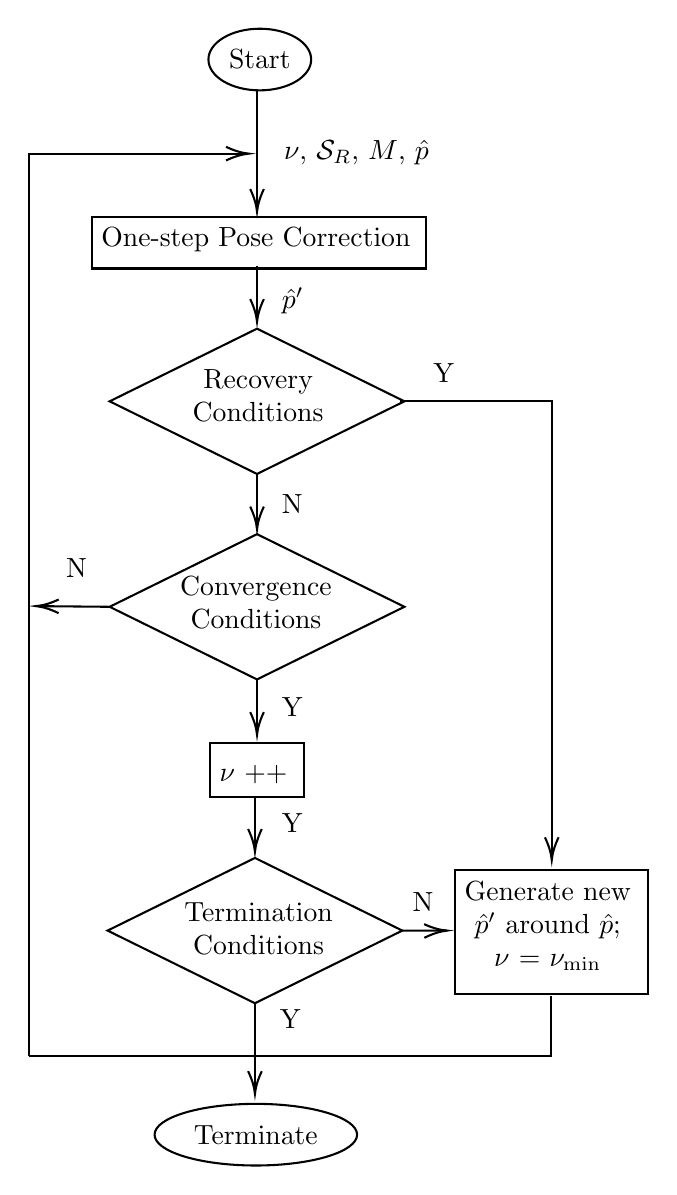
\begin{tikzpicture}[x=0.75pt,y=0.75pt,yscale=-1,xscale=1]
%uncomment if require: \path (0,1001); %set diagram left start at 0, and has height of 1001

%Flowchart: Decision [id:dp5485531374796404]
\draw   (240.5,167) -- (311.5,202) -- (240.5,237) -- (169.5,202) -- cycle ;
%Straight Lines [id:da5877536487984554]
\draw    (240.5,52.67) -- (240.5,108.67) ;
\draw [shift={(240.5,110.67)}, rotate = 270] [color={rgb, 255:red, 0; green, 0; blue, 0 }  ][line width=0.75]    (10.93,-3.29) .. controls (6.95,-1.4) and (3.31,-0.3) .. (0,0) .. controls (3.31,0.3) and (6.95,1.4) .. (10.93,3.29)   ;
%Straight Lines [id:da7274819726754627]
\draw    (240.5,237) -- (240.5,261.67) ;
\draw [shift={(240.5,263.67)}, rotate = 270] [color={rgb, 255:red, 0; green, 0; blue, 0 }  ][line width=0.75]    (10.93,-3.29) .. controls (6.95,-1.4) and (3.31,-0.3) .. (0,0) .. controls (3.31,0.3) and (6.95,1.4) .. (10.93,3.29)   ;
%Straight Lines [id:da7064477442798851]
\draw    (309.5,202) -- (382.5,202) -- (382.5,422) ;
\draw [shift={(382.5,423)}, rotate = 270.0] [color={rgb, 255:red, 0; green, 0; blue, 0 }  ][line width=0.75]    (10.93,-3.29) .. controls (6.95,-1.4) and (3.31,-0.3) .. (0,0) .. controls (3.31,0.3) and (6.95,1.4) .. (10.93,3.29)   ;
%Flowchart: Decision [id:dp1133428099178595]
\draw   (240.5,266) -- (311.5,301) -- (240.5,336) -- (169.5,301) -- cycle ;
%Flowchart: Decision [id:dp5073654995853492]
\draw   (239.5,422) -- (310.5,457) -- (239.5,492) -- (168.5,457) -- cycle ;
%Straight Lines [id:da1335991408375894]
\draw    (239.5,492) -- (239.5,533.67) ;
\draw [shift={(239.5,535.67)}, rotate = 270] [color={rgb, 255:red, 0; green, 0; blue, 0 }  ][line width=0.75]    (10.93,-3.29) .. controls (6.95,-1.4) and (3.31,-0.3) .. (0,0) .. controls (3.31,0.3) and (6.95,1.4) .. (10.93,3.29)   ;
%Straight Lines [id:da5471544644867792]
\draw    (234.5,82.67) -- (130.5,82.67) -- (130.5,517.33) ;
\draw [shift={(236.5,82.67)}, rotate = 180] [color={rgb, 255:red, 0; green, 0; blue, 0 }  ][line width=0.75]    (10.93,-3.29) .. controls (6.95,-1.4) and (3.31,-0.3) .. (0,0) .. controls (3.31,0.3) and (6.95,1.4) .. (10.93,3.29)   ;
%Straight Lines [id:da06493806045400974]
\draw    (310.5,457) -- (329,457.03) -- (332,457.03) ;
\draw [shift={(332,457)}, rotate = 539.01] [color={rgb, 255:red, 0; green, 0; blue, 0 }  ][line width=0.75]    (10.93,-3.29) .. controls (6.95,-1.4) and (3.31,-0.3) .. (0,0) .. controls (3.31,0.3) and (6.95,1.4) .. (10.93,3.29)   ;
%Straight Lines [id:da02699596164541651]
\draw    (240.5,137) -- (240.5,161.67) ;
\draw [shift={(240.5,163.67)}, rotate = 270] [color={rgb, 255:red, 0; green, 0; blue, 0 }  ][line width=0.75]    (10.93,-3.29) .. controls (6.95,-1.4) and (3.31,-0.3) .. (0,0) .. controls (3.31,0.3) and (6.95,1.4) .. (10.93,3.29)   ;
%Straight Lines [id:da5283272652442879]
\draw    (240.5,336) -- (240.5,360.67) ;
\draw [shift={(240.5,362.67)}, rotate = 270] [color={rgb, 255:red, 0; green, 0; blue, 0 }  ][line width=0.75]    (10.93,-3.29) .. controls (6.95,-1.4) and (3.31,-0.3) .. (0,0) .. controls (3.31,0.3) and (6.95,1.4) .. (10.93,3.29)   ;
%Straight Lines [id:da11468273552980146]
\draw    (239.5,392.33) -- (239.5,417) ;
\draw [shift={(239.5,419)}, rotate = 270] [color={rgb, 255:red, 0; green, 0; blue, 0 }  ][line width=0.75]    (10.93,-3.29) .. controls (6.95,-1.4) and (3.31,-0.3) .. (0,0) .. controls (3.31,0.3) and (6.95,1.4) .. (10.93,3.29)   ;
%Straight Lines [id:da44842589807001]
\draw    (169.5,301) -- (136,300.69) ;
\draw [shift={(134,300.67)}, rotate = 360.53999999999996] [color={rgb, 255:red, 0; green, 0; blue, 0 }  ][line width=0.75]    (10.93,-3.29) .. controls (6.95,-1.4) and (3.31,-0.3) .. (0,0) .. controls (3.31,0.3) and (6.95,1.4) .. (10.93,3.29)   ;
%Straight Lines [id:da5521661750319236]
\draw    (382,488.67) -- (382,517.33) -- (130.5,517.33) ;

% Text Node
\draw    (161,113) -- (322,113) -- (322,138) -- (161,138) -- cycle  ;
\draw (164,117) node [anchor=north west][inner sep=0.75pt]   [align=center] {One-step Pose Correction};
% Text Node
\draw    (241.84, 37.33) circle [x radius= 24.75, y radius= 14.85]   ;
\draw (241.84,37.33) node   [align=left] {Start};
% Text Node
\draw (208,185) node [anchor=north west][inner sep=0.75pt]  [align=center] {Recovery\\Conditions};
% Text Node
\draw (202,285) node [anchor=north west][inner sep=0.75pt]  [align=center] {Convergence\\Conditions};
% Text Node
\draw    (336,427.67) -- (429,427.67) -- (429,487.67) -- (336,487.67) -- cycle  ;
\draw (339,431.67) node [anchor=north west][inner sep=0.75pt]  [align=center] {Generate new \\ $\hat{\bm{p}}^\prime$ around $\hat{\bm{p}}$; \\ $\nu$ = $\nu_{\min}$};
% Text Node
\draw (324,182.33) node [anchor=north west][inner sep=0.75pt]   [align=left] {Y};
% Text Node
\draw (251,245.33) node [anchor=north west][inner sep=0.75pt]   [align=left] {N};
% Text Node
\draw    (218,366.67) -- (263,366.67) -- (263,392.67) -- (218,392.67) -- cycle  ;
\draw (221,375.67) node [anchor=north west][inner sep=0.75pt]   [align=center] {$\nu$ ++};
% Text Node
\draw (251,343.33) node [anchor=north west][inner sep=0.75pt]   [align=left] {Y};
% Text Node
\draw (252,74.57) node [anchor=north west][inner sep=0.75pt]   [align=left] {$\nu$, $\mathcal{S}_R$, $\bm{M}$, $\hat{\bm{p}}$};
% Text Node
\draw (204,442) node [anchor=north west][inner sep=0.75pt] [align=center] {Termination\\Conditions};
% Text Node
\draw    (239.93, 555.33) circle [x radius= 48.79, y radius= 14.85]   ;
\draw (239.93,555.33) node   [align=left] {Terminate};
% Text Node
\draw (147,276.33) node [anchor=north west][inner sep=0.75pt]   [align=left] {N};
% Text Node
\draw (251,399.33) node [anchor=north west][inner sep=0.75pt]   [align=left] {Y};
% Text Node
\draw (314,437.33) node [anchor=north west][inner sep=0.75pt]   [align=left] {N};
% Text Node
\draw (251,145.57) node [anchor=north west][inner sep=0.75pt]   [align=left] {$\hat{\bm{p}}^\prime$};
% Text Node
\draw (250,493.33) node [anchor=north west][inner sep=0.75pt]   [align=left] {Y};


\end{tikzpicture}


  \caption{\small Το διάγραμμα ροής του FSMSM. Η εκτέλεση αρχίζει με μια αρχική
           γωνιακό βαθμό δειγματοληψίας $\nu_{\min}$, η σάρωση που καταγράφεται
           από το αισθητήρα φυσικού εύρους $\mathcal{S}_R$, και ο χάρτης του
           περιβάλλοντος $\bm{M}$. Η αρχική εκτίμηση της στάσης παρέχεται από
           ένα φίλτρο παρακολούθησης κατά τη διάρκεια της ανίχνευσης της στάσης
           ή με τη μορφή μιας υπόθεσης κατά τη διάρκεια της συνολικής
           εντοπισμού. Η εσωτερική μέθοδος One-step Pose Correction (διόρθωση
           πόζας ενός βήματος) (εικ. \ref{fig:02_04_04:inner_system}) καλείται
           επαναληπτικά, ενημερώνοντας την πόζα εκτίμηση, μέχρι να επιτευχθεί
           ένας μέγιστος βαθμός γωνιακής δειγματοληψίας}
  \label{fig:02_04_04:outer_system}
\end{figure}

Έστω οι προϋποθέσεις του προβλήματος \ref{prob:02_04}, δηλαδή
η αρχική εκτίμηση εισόδου $\hat{\bm{p}}(\hat{x}, \hat{y}, \hat{\theta})$,
η πραγματική σάρωση $\mathcal{S}_R$, και ο χάρτης $\bm{M}$. Τότε
η μέθοδος ελάττωσης του συνολικού σφάλματος εκτίμησης στάσης που προτείνουμε,
την οποία ονομάζουμε Fourier Scan--to--Map-Scan Matching (FSMSM) και η οποία
παρουσιάζεται στο σχήμα \ref{fig:02_04_04:outer_system},---η μέθοδος μειώνει το
σφάλμα με την επαναληπτική εκτέλεση της διαδικασίας ελάττωσης σφάλματος ενός
βήματος (One-step Pose Correction, OPC---σχήμα \ref{fig:02_04_04:inner_system}),
μέχρι να ικανοποιηθεί ένα σύνολο συνθηκών τερματισμού. Η FSMSM ξεκινά με ένα
αρχικό βαθμό δειγματοληψίας του χάρτη $\nu$ = $\nu_{\min}$. Η εκτίμηση της
στάσης εισόδου επεξεργάζεται από την OPC, και η έξοδός της
$\hat{\bm{p}}^\prime$ εξετάζεται ως προς συνθήκες ανάκτησης και
σύγκλισης. Εάν η προκύπτουσα εκτίμηση στάσης βρεθεί εκτός του χάρτη $\bm{M}$
τότε δημιουργείται μια νέα εκτίμηση από την αρχική
εκτίμηση, και η διαδικασία επανεκιννεί. Εάν δεν παρατηρείται σημαντική
διόρθωση της εκτίμησης
$\|\hat{\bm{p}}^\prime-\hat{\bm{p}}\|_2 < \varepsilon_{\delta p}$, τότε ο
βαθμός δειγματοληψίας του χάρτη $\nu$ αυξάνεται. Η αύξησή του χρησιμεύει ως
μέσο μείωσης του σφάλματος προσανατολισμού και συνεπώς του σφάλματος εκτίμησης
θέσης (Παρατήρηση \ref{remark:loc_prop_or}). Διαφορετικά, η διαδικασία
διόρθωσης της στάσης σε ένα βήμα είναι η εξής επαναλαμβάνεται έως ότου δεν
παρατηρηθεί σημαντική διόρθωση. Η διαδικασία επαναλαμβάνεται έως ότου
επιτευχθεί ο μέγιστος βαθμός δειγματοληψίας χάρτη $\nu$ = $\nu_{\max}$, σε
οπότε το FSMSM τερματίζει εάν πληρούται μια τελική συνθήκη. Αυτή η τελική
συνθήκη διευκολύνει την αποφυγή τοπικών μεγίστων. Στην περίπτωση που αυτό το
συνθήκη δεν ικανοποιείται, δημιουργείται μια νέα πόζα και η διαδικασία
επαναφέρεται.

\begin{figure}[h]\centering
  

\tikzset{every picture/.style={line width=0.75pt}} %set default line width to 0.75pt

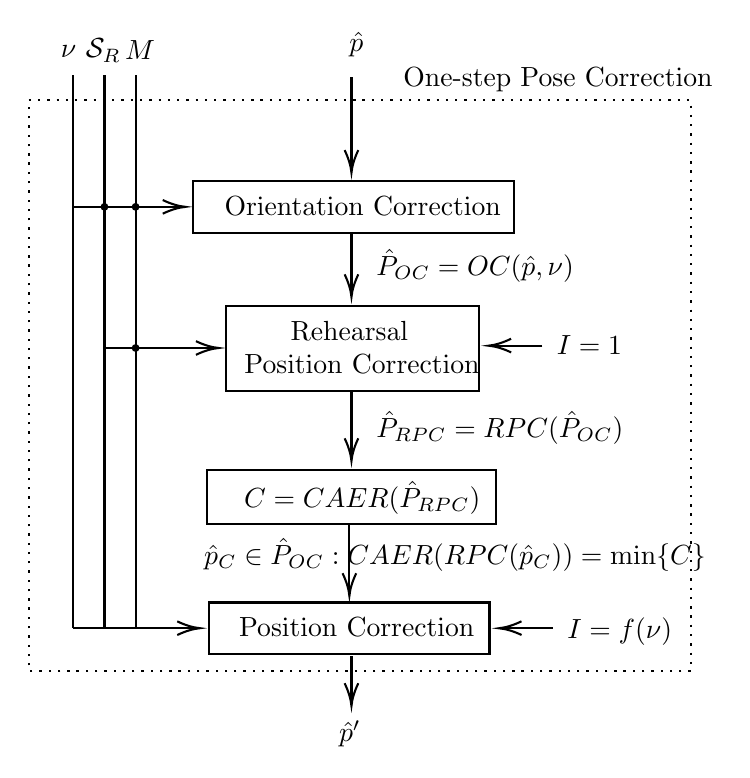
\begin{tikzpicture}[x=0.75pt,y=0.75pt,yscale=-1,xscale=1]
%uncomment if require: \path (0,542); %set diagram left start at 0, and has height of 542

%Straight Lines [id:da5372026622110897]
\draw    (126.5,63) -- (126.5,329.29) ;
%Straight Lines [id:da7972290663823844]
\draw    (260.5,64) -- (260.5,108) ;
\draw [shift={(260.5,110)}, rotate = 270] [color={rgb, 255:red, 0; green, 0; blue, 0 }  ][line width=0.75]    (10.93,-3.29) .. controls (6.95,-1.4) and (3.31,-0.3) .. (0,0) .. controls (3.31,0.3) and (6.95,1.4) .. (10.93,3.29)   ;
%Straight Lines [id:da2357744220142839]
\draw    (260.5,138.86) -- (260.5,167.86) ;
\draw [shift={(260.5,169.86)}, rotate = 270] [color={rgb, 255:red, 0; green, 0; blue, 0 }  ][line width=0.75]    (10.93,-3.29) .. controls (6.95,-1.4) and (3.31,-0.3) .. (0,0) .. controls (3.31,0.3) and (6.95,1.4) .. (10.93,3.29)   ;
%Straight Lines [id:da9232696254114303]
\draw    (352.5,193.29) -- (328.5,193.29) ;
\draw [shift={(326.5,193.29)}, rotate = 359.69] [color={rgb, 255:red, 0; green, 0; blue, 0 }  ][line width=0.75]    (10.93,-3.29) .. controls (6.95,-1.4) and (3.31,-0.3) .. (0,0) .. controls (3.31,0.3) and (6.95,1.4) .. (10.93,3.29)   ;
%Straight Lines [id:da7890748320756154]
\draw    (259.5,278.86) -- (259.5,311.86) ;
\draw [shift={(259.5,313.86)}, rotate = 270] [color={rgb, 255:red, 0; green, 0; blue, 0 }  ][line width=0.75]    (10.93,-3.29) .. controls (6.95,-1.4) and (3.31,-0.3) .. (0,0) .. controls (3.31,0.3) and (6.95,1.4) .. (10.93,3.29)   ;
%Straight Lines [id:da3579629949332166]
\draw    (260.5,342.86) -- (260.5,364.86) ;
\draw [shift={(260.5,366.86)}, rotate = 270] [color={rgb, 255:red, 0; green, 0; blue, 0 }  ][line width=0.75]    (10.93,-3.29) .. controls (6.95,-1.4) and (3.31,-0.3) .. (0,0) .. controls (3.31,0.3) and (6.95,1.4) .. (10.93,3.29)   ;
%Straight Lines [id:da8737381615370248]
\draw    (141.5,63) -- (141.5,329.29) ;
%Straight Lines [id:da6971384120103545]
\draw    (156.5,63) -- (156.5,329.29) ;
%Straight Lines [id:da8422749343405824]
\draw    (178.5,126.4) -- (156.5,126.4) ;
\draw [shift={(156.5,126.4)}, rotate = 180] [color={rgb, 255:red, 0; green, 0; blue, 0 }  ][fill={rgb, 255:red, 0; green, 0; blue, 0 }  ][line width=0.75]      (0, 0) circle [x radius= 1.35, y radius= 1.35]   ;
\draw [shift={(180.5,126.4)}, rotate = 180] [color={rgb, 255:red, 0; green, 0; blue, 0 }  ][line width=0.75]    (10.93,-3.29) .. controls (6.95,-1.4) and (3.31,-0.3) .. (0,0) .. controls (3.31,0.3) and (6.95,1.4) .. (10.93,3.29)   ;
%Straight Lines [id:da4007753539436163]
\draw    (156.5,126.4) -- (141.5,126.4) ;
\draw [shift={(141.5,126.4)}, rotate = 180] [color={rgb, 255:red, 0; green, 0; blue, 0 }  ][fill={rgb, 255:red, 0; green, 0; blue, 0 }  ][line width=0.75]      (0, 0) circle [x radius= 1.35, y radius= 1.35]   ;
%Straight Lines [id:da579363628601445]
\draw    (141.5,126.4) -- (126.5,126.4) ;
%Straight Lines [id:da5833842782446357]
\draw    (357.5,329.43) -- (333.5,329.43) ;
\draw [shift={(331.5,329.43)}, rotate = 359.69] [color={rgb, 255:red, 0; green, 0; blue, 0 }  ][line width=0.75]    (10.93,-3.29) .. controls (6.95,-1.4) and (3.31,-0.3) .. (0,0) .. controls (3.31,0.3) and (6.95,1.4) .. (10.93,3.29)   ;
%Straight Lines [id:da7806442385955334]
\draw    (260.5,214.86) -- (260.5,246.86) ;
\draw [shift={(260.5,248.86)}, rotate = 270] [color={rgb, 255:red, 0; green, 0; blue, 0 }  ][line width=0.75]    (10.93,-3.29) .. controls (6.95,-1.4) and (3.31,-0.3) .. (0,0) .. controls (3.31,0.3) and (6.95,1.4) .. (10.93,3.29)   ;
%Straight Lines [id:da6458571735202372]
\draw    (194.5,194.4) -- (156.5,194.4) ;
\draw [shift={(156.5,194.4)}, rotate = 180] [color={rgb, 255:red, 0; green, 0; blue, 0 }  ][fill={rgb, 255:red, 0; green, 0; blue, 0 }  ][line width=0.75]      (0, 0) circle [x radius= 1.35, y radius= 1.35]   ;
\draw [shift={(196.5,194.4)}, rotate = 180] [color={rgb, 255:red, 0; green, 0; blue, 0 }  ][line width=0.75]    (10.93,-3.29) .. controls (6.95,-1.4) and (3.31,-0.3) .. (0,0) .. controls (3.31,0.3) and (6.95,1.4) .. (10.93,3.29)   ;
%Straight Lines [id:da3539392704501798]
\draw    (156.5,194.5) -- (141.5,194.5) ;
%Straight Lines [id:da41656320353747733]
\draw    (185.5,329.4) -- (126.5,329.4) ;
\draw [shift={(187.5,329.4)}, rotate = 180] [color={rgb, 255:red, 0; green, 0; blue, 0 }  ][line width=0.75]    (10.93,-3.29) .. controls (6.95,-1.4) and (3.31,-0.3) .. (0,0) .. controls (3.31,0.3) and (6.95,1.4) .. (10.93,3.29)   ;
%Shape: Rectangle [id:dp8185193791005427]
\draw  [dash pattern={on 0.84pt off 2.51pt}] (105,75) -- (424,75) -- (424,350) -- (105,350) -- cycle ;
\draw (360,65) node  {One-step Pose Correction};

% Text Node
\draw    (184,114) -- (339,114) -- (339,139) -- (184,139) -- cycle  ;
\draw (189,120) node [anchor=north west][inner sep=0.75pt]   [align=left] {\ \ Orientation Correction};
% Text Node
\draw (119,47) node [anchor=north west][inner sep=0.75pt]   [align=left] {$\nu$};
% Text Node
\draw (131,44) node [anchor=north west][inner sep=0.75pt]   [align=left] {$\mathcal{S}_{R}$};
% Text Node
\draw (258,40.57) node [anchor=north west][inner sep=0.75pt]   [align=left] {$\hat{\bm{p}}$};
% Text Node
\draw (150,44.57) node [anchor=north west][inner sep=0.75pt]   [align=left] {$\bm{M}$};
% Text Node
\draw  [color={rgb, 255:red, 0; green, 0; blue, 0 }  ,draw opacity=1 ]  (200,174) -- (322,174) -- (322,215) -- (200,215) -- cycle  ;
\draw (203,180) node [anchor=north west][inner sep=0.75pt]  [align=left] {\ \ \ \ \ \ Rehearsal \\ \ Position Correction};
% Text Node
\draw    (191,253) -- (330,253) -- (330,279) -- (191,279) -- cycle  ;
\draw (194,257) node [anchor=north west][inner sep=0.75pt]   [align=left] {\ \ \ $\bm{C} = \text{CAER}(\hat{\bm{P}}_{RPC})$};
% Text Node
\draw (358,187) node [anchor=north west][inner sep=0.75pt]   [align=left] {$I = 1$};
% Text Node
\draw    (192,317) -- (327,317) -- (327,342) -- (192,342) -- cycle  ;
\draw (196,323) node [anchor=north west][inner sep=0.75pt]   [align=left] {\ \ Position Correction};
% Text Node
\draw (253,372.67) node [anchor=north west][inner sep=0.75pt]   [align=left] {$\hat{\bm{p}}^{\prime }$};
% Text Node
\draw (271,145.5) node [anchor=north west][inner sep=0.75pt]   [align=left] {$\hat{\bm{P}}_{OC} = \text{OC}(\hat{\bm{p}}, \nu)$};
% Text Node
\draw (363,323) node [anchor=north west][inner sep=0.75pt]   [align=left] {$I = f( \nu )$};
% Text Node
\draw (271,223.5) node [anchor=north west][inner sep=0.75pt]   [align=left] {$\hat{\bm{P}}_{RPC} = \text{RPC}(\hat{\bm{P}}_{OC})$};
% Text Node
\draw (188,284.5) node [anchor=north west][inner sep=0.75pt]   [align=left] {$\hat{\bm{p}}_{C} \in \hat{\bm{P}}_{OC} : \text{CAER}(\text{RPC}(\hat{\bm{p}}_C)) = \min\{\bm{C}\}$};


\end{tikzpicture}


  \caption{\small  βασική μέθοδος ευθυγράμμισης πόζας του FSMSM, που ονομάζεται
           One-step Pose Correction}
  \label{fig:02_04_04:inner_system}
\end{figure}


Δεδομένης μιας εκτίμησης πόζας εισόδου $\hat{\bm{p}}(\hat{x}, \hat{y},
\hat{\theta})$, η πραγματική σάρωση $\mathcal{S}_R$, ο χάρτης $\bm{M}$ και ένας
βαθμός δειγματοληψίας $\nu$, το σύστημα διόρθωσης πόζας ενός βήματος υπολογίζει
πρώτα εκτιμήσεις πόζας $2^\nu$ $\hat{\bm{P}}_{OC} = \{(\hat{x}, \hat{y},
\hat{\theta}_k)\}$, $k = 0,\dots,2^\nu$$-$$1$. Το σύστημα διόρθωσης
προσανατολισμού χρησιμοποιεί τον αλγόριθμο \ref{alg:algorithm_ufrcnu}. Η
λειτουργία του συμβολίζεται στο σχήμα.  \ref{fig:02_04_04:inner_system} με τον τελεστή
OC$(\cdot)$.

Τώρα, εάν η θέση της εκτίμησης της πόζας εισόδου συμπίπτει με τη θέση του του
πραγματικού αισθητήρα, η μετρική Percent Discrimination (εξ. \ref{eq:pd}) θα
αρκούσε για να χρησιμεύσει ως ακριβής προσδιοριστής της εκτίμησης της πόζας με
τον ελάχιστο σφάλμα προσανατολισμού. Στην πράξη, ωστόσο, η κατάταξη που
παρέχεται από την Percent Discrimination μετρική, μπερδεύεται από την ασυνέπεια
των δύο θέσεων.  Προκειμένου να αμβλυνθεί αυτό το φαινόμενο, κάθε εκτίμηση
στάσης στο $\hat{\bm{P}}_{OC}$ δίνεται στο σύστημα διόρθωσης θέσης, όπου η θέση
κάθε εκτίμησης πόζας μετατοπίζεται μία φορά ($I$=$1$), σύμφωνα με την
Αλγόριθμος \ref{alg:algorithm_icte}. Αυτή η λειτουργία, που συμβολίζεται με τον
τελεστή RPC$(\cdot)$ στην εικ. \ref{fig:02_04_04:inner_system}, παράγει το σύνολο
$\hat{\bm{P}}_{RPC} = \{(\hat{x}_k, \hat{y}_k, \hat{\theta}_k)\}$,
$|\hat{\bm{P}}_{RPC}| = 2^\nu$.  Ο σκοπός αυτής της πράξης είναι να να παρέχει
μια εκ των προτέρων εικόνα του επόμενου βήματος της διόρθωσης της θέσης: το
λιγότερο περιστροφικά κακή ευθυγράμμιση είναι μια εκτίμηση της στάσης, τόσο
λιγότερο θα αποκλίνει ως προς την προσανατολισμού και συνεπώς της θέσης σε
σχέση με την πραγματική θέση του αισθητήρα μόλις εισάγεται στο σύστημα
διόρθωσης θέσης (παρατήρηση \ref{remark:loc_prop_or}).  Αυτή η απόκλιση
αποτυπώνεται από το αθροιστικό απόλυτο σφάλμα ανά ακτίνα (CAER) μετρική:
\begin{align}
  \text{CAER}_k = & \sum\limits_{n=0}^{N_s-1} \Bigg| \mathcal{S}_R[n] - \mathcal{S}_V[n]\Big|_{(\hat{x}_k, \hat{y}_k, \hat{\theta}_k)} \Bigg|
  \label{eq:caer}
\end{align}
όπου $k$ = $0,\dots,2^\nu$$-$$1$. Η μετρική CAER (εικ. \ref{fig:02_04_04:caer})
κωδικοποιεί ταυτόχρονα ένα βαθμό ευθυγράμμισης της θέσης και του
προσανατολισμού μεταξύ των δύο σαρώσεων εισόδου της.\footnote{Αντίθετα, η
αφαίρεση της απόλυτης τιμής θα παρείχε μόνο μια μετρική ευθυγράμμισης θέσης.}
Με την επανάληψη του διόρθωση θέσης κάθε εκτίμησης της θέσης στο
$\hat{\bm{P}}_{OC}$ και την καταγραφή την CAER για κάθε μια από τις
μετατοπισμένες εκτιμήσεις πόζας στο $\hat{\bm{P}_{RPC}}$, είναι είναι δυνατόν
να καθοριστεί μια κατάταξη σφάλματος πόζας μεταξύ των εκτιμήσεων πόζας στο
$\hat{\bm{P}}_{OC}$ και ταυτόχρονα να διατηρείται μόνο μία εκτίμηση πόζας για
την την επόμενη επανάληψη της μεθόδου διόρθωσης πόζας ενός
βήματος.\footnote{Αλλιώς, η διόρθωση της θέσης των εκτιμήσεων πόζας $2^\nu$ και
η επανατροφοδότησή τους στην διόρθωση πόζας ενός βήματος θα προκαλούσε εκθετικό
κόστος σε χρόνο εκτέλεσης.} Η εκτίμηση πόζας $\hat{\bm{p}}_C \in
\hat{\bm{P}}_{OC}$ η οποία, όταν μεταφράζεται μία φορά, καταγράφει το ελάχιστο
CAER μεταξύ όλων των παρόμοια επεξεργασμένων πόζων εκτιμήσεις στο
$\hat{\bm{P}}_{OC}$ εισάγεται στη μέθοδο διόρθωσης θέσης proper. Ο αριθμός των
επαναλήψεων μετάφρασης $I$ που υφίσταται είναι ένας αυξανόμενος συνάρτηση του
βαθμού δειγματοληψίας του χάρτη $\nu$.\footnote{Η λογική της αλυσιδωτής
σύνδεσης του αριθμού των μεταφραστικών επαναλήψεων με το βαθμό δειγματοληψίας
του χάρτη $\nu$ είναι η ακόλουθη.  Δεδομένου ότι το σφάλμα προσανατολισμού
είναι αντιστρόφως ανάλογο με το $\nu$, σε χαμηλούς βαθμούς δειγματοληψίας
χάρτη, όταν το σφάλμα εκτίμησης θέσης είναι στο υψηλότερο, εάν ο αριθμός των
μεταφραστικών επαναλήψεων ήταν υψηλός, τότε η θέση εκτίμηση της θέσης θα ήταν
ευάλωτη σε απόκλιση. Επομένως, ο αριθμός των μεταφραστικών επαναλήψεων
διατηρείται χαμηλός στα αρχικά στάδια έτσι ώστε να υπάρχει ισορροπία μεταξύ της
μείωσης του σφάλματος θέσης και της απόκλισης θέσης. Σε υψηλότερα τιμές του
$\nu$, το σφάλμα εκτίμησης προσανατολισμού μειώνεται και στη συνέχεια η
απόκλιση περιορίζεται ή/και ικανοποιείται σε υψηλότερες τιμές μεταφραστικής
επανάληψης.  Καθώς η εκτίμηση προσανατολισμού γίνεται όλο και πιο ακριβής, το
σύστημα διόρθωσης θέσης αφήνεται να επαναλάβει περισσότερες φορές, ώστε να
μειωθεί περαιτέρω το σφάλμα θέσης να είναι εφικτό.} Το σύστημα διόρθωσης θέσης
παράγει $\hat{\bm{p}}^\prime$, το οποίο στη συνέχεια τροφοδοτείται πίσω στο
σύστημα διόρθωσης προσανατολισμού με τη μορφή του νέου του εκτίμησης της θέσης
$\hat{\bm{p}} \leftarrow \hat{\bm{p}}^\prime$. Στην πράξη, η σύνολο πόζας
$\hat{\bm{P}}_{OC}$ συμπληρώνεται με μία πόζα της οποίας η θέση είναι ίση με
$\hat{\bm{p}}$ και του οποίου ο προσανατολισμός είναι ίσος με τον
προσανατολισμό του $\hat{\bm{p}}_C$ που παράγει το ελάχιστο CAER με την πάροδο
του χρόνου. Αυτή η προσθήκη εισάγει μια μορφή μνήμης στο σύστημα, η οποία το
βοηθά στην αποφυγή απόκλιση και η οποία, ως εκ τούτου, ωφελεί την ταχύτητα
εκτέλεσης.


\begin{figure}[h]\centering
  % GNUPLOT: LaTeX picture with Postscript
\begingroup
  \makeatletter
  \providecommand\color[2][]{%
    \GenericError{(gnuplot) \space\space\space\@spaces}{%
      Package color not loaded in conjunction with
      terminal option `colourtext'%
    }{See the gnuplot documentation for explanation.%
    }{Either use 'blacktext' in gnuplot or load the package
      color.sty in LaTeX.}%
    \renewcommand\color[2][]{}%
  }%
  \providecommand\includegraphics[2][]{%
    \GenericError{(gnuplot) \space\space\space\@spaces}{%
      Package graphicx or graphics not loaded%
    }{See the gnuplot documentation for explanation.%
    }{The gnuplot epslatex terminal needs graphicx.sty or graphics.sty.}%
    \renewcommand\includegraphics[2][]{}%
  }%
  \providecommand\rotatebox[2]{#2}%
  \@ifundefined{ifGPcolor}{%
    \newif\ifGPcolor
    \GPcolorfalse
  }{}%
  \@ifundefined{ifGPblacktext}{%
    \newif\ifGPblacktext
    \GPblacktexttrue
  }{}%
  % define a \g@addto@macro without @ in the name:
  \let\gplgaddtomacro\g@addto@macro
  % define empty templates for all commands taking text:
  \gdef\gplfronttext{}%
  \gdef\gplfronttext{}%
  \makeatother
  \ifGPblacktext
    % no textcolor at all
    \def\colorrgb#1{}%
    \def\colorgray#1{}%
  \else
    % gray or color?
    \ifGPcolor
      \def\colorrgb#1{\color[rgb]{#1}}%
      \def\colorgray#1{\color[gray]{#1}}%
      \expandafter\def\csname LTw\endcsname{\color{white}}%
      \expandafter\def\csname LTb\endcsname{\color{black}}%
      \expandafter\def\csname LTa\endcsname{\color{black}}%
      \expandafter\def\csname LT0\endcsname{\color[rgb]{1,0,0}}%
      \expandafter\def\csname LT1\endcsname{\color[rgb]{0,1,0}}%
      \expandafter\def\csname LT2\endcsname{\color[rgb]{0,0,1}}%
      \expandafter\def\csname LT3\endcsname{\color[rgb]{1,0,1}}%
      \expandafter\def\csname LT4\endcsname{\color[rgb]{0,1,1}}%
      \expandafter\def\csname LT5\endcsname{\color[rgb]{1,1,0}}%
      \expandafter\def\csname LT6\endcsname{\color[rgb]{0,0,0}}%
      \expandafter\def\csname LT7\endcsname{\color[rgb]{1,0.3,0}}%
      \expandafter\def\csname LT8\endcsname{\color[rgb]{0.5,0.5,0.5}}%
    \else
      % gray
      \def\colorrgb#1{\color{black}}%
      \def\colorgray#1{\color[gray]{#1}}%
      \expandafter\def\csname LTw\endcsname{\color{white}}%
      \expandafter\def\csname LTb\endcsname{\color{black}}%
      \expandafter\def\csname LTa\endcsname{\color{black}}%
      \expandafter\def\csname LT0\endcsname{\color{black}}%
      \expandafter\def\csname LT1\endcsname{\color{black}}%
      \expandafter\def\csname LT2\endcsname{\color{black}}%
      \expandafter\def\csname LT3\endcsname{\color{black}}%
      \expandafter\def\csname LT4\endcsname{\color{black}}%
      \expandafter\def\csname LT5\endcsname{\color{black}}%
      \expandafter\def\csname LT6\endcsname{\color{black}}%
      \expandafter\def\csname LT7\endcsname{\color{black}}%
      \expandafter\def\csname LT8\endcsname{\color{black}}%
    \fi
  \fi
    \setlength{\unitlength}{0.0500bp}%
    \ifx\gptboxheight\undefined%
      \newlength{\gptboxheight}%
      \newlength{\gptboxwidth}%
      \newsavebox{\gptboxtext}%
    \fi%
    \setlength{\fboxrule}{0.5pt}%
    \setlength{\fboxsep}{1pt}%
\begin{picture}(10000.00,4000.00)%
    \gplgaddtomacro\gplfronttext{%
    }%
    \gplgaddtomacro\gplfronttext{%
      \colorrgb{0.15,0.15,0.15}%
      \put(135,1003){\makebox(0,0)[r]{\strut{}$0.05$}}%
      \colorrgb{0.15,0.15,0.15}%
      \put(135,1571){\makebox(0,0)[r]{\strut{}$0.10$}}%
      \colorrgb{0.15,0.15,0.15}%
      \put(135,2137){\makebox(0,0)[r]{\strut{}$0.15$}}%
      \colorrgb{0.15,0.15,0.15}%
      \put(135,2705){\makebox(0,0)[r]{\strut{}$0.20$}}%
      \colorrgb{0.15,0.15,0.15}%
      \put(135,3273){\makebox(0,0)[r]{\strut{}$0.25$}}%
      \colorrgb{0.15,0.15,0.15}%
      \put(-700,600){\rotatebox{90}{\strut{}Σφάλμα θέσης $(\Delta x^2 + \Delta y^2)^{1/2}$}}%
      \colorrgb{0.15,0.15,0.15}%
      \put(301,164){\makebox(0,0){\strut{}$ -\dfrac{\pi}{4}$}}%
      \colorrgb{0.15,0.15,0.15}%
      \put(1301,164){\makebox(0,0){\strut{}$ -\dfrac{\pi}{8}$}}%
      \colorrgb{0.15,0.15,0.15}%
      \put(1801,164){\makebox(0,0){\strut{}$ -\dfrac{\pi}{16}$}}%
      \colorrgb{0.15,0.15,0.15}%
      \put(2300,164){\makebox(0,0){\strut{} $0.0$}}%
      \colorrgb{0.15,0.15,0.15}%
      \put(2799,164){\makebox(0,0){\strut{}$ +\dfrac{\pi}{16}$}}%
      \colorrgb{0.15,0.15,0.15}%
      \put(3299,164){\makebox(0,0){\strut{}$ +\dfrac{\pi}{8}$}}%
      \colorrgb{0.15,0.15,0.15}%
      \put(4299,164){\makebox(0,0){\strut{}$ +\dfrac{\pi}{4}$}}%
      \colorrgb{0.15,0.15,0.15}%
      \put(2300,-360){\makebox(0,0){\strut{}Σφάλμα προσανατολισμού $\Delta\theta$}}%
    }%
    \gplgaddtomacro\gplfronttext{%
    }%
    \gplgaddtomacro\gplfronttext{%
      \colorrgb{0.15,0.15,0.15}%
      \put(5674,164){\makebox(0,0){\strut{}$0.05$}}%
      \colorrgb{0.15,0.15,0.15}%
      \put(6354,164){\makebox(0,0){\strut{}$0.10$}}%
      \colorrgb{0.15,0.15,0.15}%
      \put(7033,164){\makebox(0,0){\strut{}$0.15$}}%
      \colorrgb{0.15,0.15,0.15}%
      \put(7713,164){\makebox(0,0){\strut{}$0.20$}}%
      \colorrgb{0.15,0.15,0.15}%
      \put(8393,164){\makebox(0,0){\strut{}$0.25$}}%
      \colorrgb{0.15,0.15,0.15}%
      \put(6916,-360){\makebox(0,0){\strut{}Σφάλμα θέσης $(\Delta x^2 + \Delta y^2)^{1/2}$}}%
      \colorrgb{0.15,0.15,0.15}%
      \put(4674,1400){\rotatebox{90}{\strut{}CAER [m]}}
    }%
    \gplgaddtomacro\gplfronttext{%
      \colorrgb{0.00,0.00,0.00}%
      \put(9531,460){\makebox(0,0)[l]{\strut{} $0.0$}}%
      \colorrgb{0.15,0.15,0.15}%
      \put(9531,1100){\makebox(0,0)[l]{\strut{} $100.0$}}%
      \colorrgb{0.15,0.15,0.15}%
      \put(9531,1740){\makebox(0,0)[l]{\strut{} $200.0$}}%
      \colorrgb{0.15,0.15,0.15}%
      \put(9531,2379){\makebox(0,0)[l]{\strut{} $300.0$}}%
      \colorrgb{0.15,0.15,0.15}%
      \put(9531,3019){\makebox(0,0)[l]{\strut{} $400.0$}}%
      \colorrgb{0.15,0.15,0.15}%
      \put(9531,3659){\makebox(0,0)[l]{\strut{} $500.0$}}%
    }%
    \put(0,0){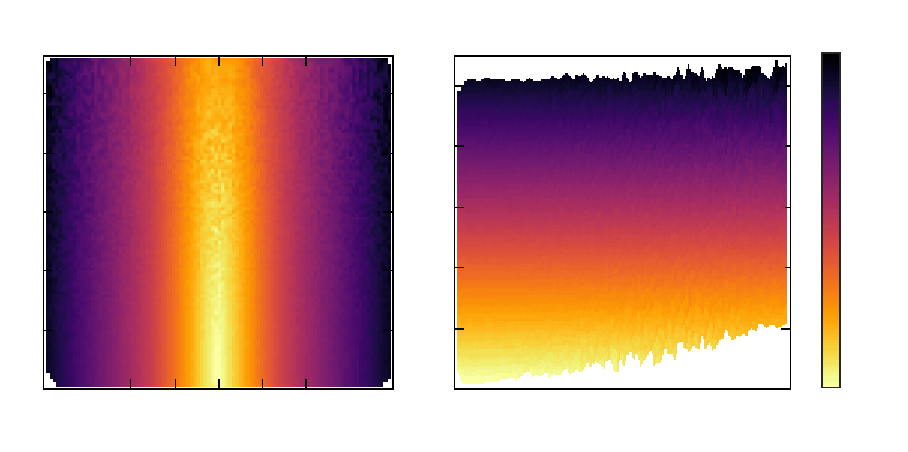
\includegraphics{./figures/parts/02/chapters/04/sections/04/caer_x2}}%
    \gplfronttext
  \end{picture}%
\endgroup

  \vspace{1cm}
  \caption{\small Ένα προφίλ της μετρικής CAER (eq. (\ref{eq:caer})) από το
           $10^6$ ζεύγη δειγματοληπτικών σαρώσεων, ανάλογα με την απόσταση
           $(\Delta x^2 + \Delta y^2)^{1/2}$ και του σχετικού προσανατολισμού
           $\Delta \theta$ των θέσεων από όπου μια πραγματική και μια εικονική
           σάρωση καταγράφηκαν. Οι εκτιμήσεις πόζας που είναι πιο κοντά στην
           πραγματική πόζα από την άποψη των προσανατολισμού (α) παρουσιάζουν
           χαμηλότερες τιμές CAER από εκείνες που απέχουν περισσότερο.  από
           αυτήν και (β) παράγουν χαμηλότερα σφάλματα θέσης μόλις εισαχθούν στο
           Σύστημα διόρθωσης θέσης}
  \label{fig:02_04_04:caer}
\end{figure}
